
\chapter{Concept and Design}
\label{cha:conceptanddesign}

\section{General}

\section{Requirements and Challenges}

\subsection{Requirements}

\subsubsection{GDPR compliance}
\label{subsubsec:GDPR_compliance}
The General Data Protection Regulation (GDPR) is a regulation by the European Parliament, Council of the European Union and the European Commission focused on strengthening EU citizens digital privacy.  Its main focus is on giving citizens control over their digital personal information and simplifying the regulatory environment for multinational corporations. However it also adds a strict data compliance regime, by penalizing transgressions with up to 4\% worldwide turnover\cite{gdpr}. Furthermore this regulation does not have to be verified by each EU's regulatory body, since it is a EU regulation, compared to an EU directive which has to be ratified by each EU signatory state.

\section{Challenges}
\label{sec:challenges}

\subsection{Security Goals}
\label{sec:securityGoals}

Designing an identity management system comes with various legal implications. More specifically we are referring to § 9 “Technical and organizational actions” in the “Federal Data Protection Act”\footnote{Translated from the german version of the  “Bundesdatenschutzgesetz”} were an identity management system shall enforce all necessary measures to protect identity information.\cite{bdsg}

So we will focus on the following security goals:
\begin{enumerate}
\item \textbf{Confidentiality:} Data shall be secured on its transmission. This includes the blockchain and communication over the internet. 
\item \textbf{Integrity:} The integrity of the data needs to be assured so that no entity can change identity information without knowledge. 
\item \textbf{Authenticity:} Identity information is protected against unauthorized access. 
\item \textbf{Non-Repudiation:} No entity can deny having taken an action.
\item \textbf{Privacy:} The privacy of a user is preserved while interacting with the system. 
\end{enumerate}

We further also view the blockchain as a public ledger were everyone can read transactions or information stored on the blockchain. So interactions with the blockchain need to ensure to not expose any identity information. 
It is not allowed to store hashes or encrypted claims in the blockchain, since it is a tamper-proof data storage, once written information can not be removed or changed. So if the hash or encryption gets broken the identity information is leaked and can not be deleted from the blockchain.  

\subsection{User Acceptance}
\label{sec:userAcceptance}

Switching from offline to online identity is an unspecified burden that falls into the common eye.
Especially for the elderly and uneducated the imagination of not having a piece of paper with an id and not having a central
institution that takes care of one's identity is suspect, if not horrifying.
Not only the lack of a trusted party but also the concept of blockchain, smart contracts and all of its gists are unknown
to most people. This leads to further distrust in the system.

By introducing such a system, a lot of clarification for non-technical people and common folks therefore needs to have a
high priority.

Without understanding the process and system, users run the risk of being exploited and not being aware of what information
they are currently sharing.

\subsection{Economic feasibility}
\label{sec:economicFeasibility}
In order for a new system to become successful, it is imperative that it is economically feasible. Its total cost of ownership should be comparable to or even lower than the system it is replacing.
However, the total cost of ownership of an identity system where the blockchain is used for storing transactional information is extremely difficult to gauge. This is in part because it is a "living platform" which is constantly being changed, but also because of the volatility of cryptocurrencies.\cite{elendner2016cross}
Due to cryptos nature it is difficult to keep costs stable or predictable, since accurate models are still actively being worked on.\cite{catania2018predicting} The slightest change in financial regulation, bad press, or just negative comments in social media can crash their prices.\cite{kim2016predicting}
In contrast their prices can also rise in an astonishing fashion because of aforementioned reasons. 
This projects aim however has not been to create an economically feasible platform, but a simple demonstrator, showcasing that blockchain technologies could be adapted to suit the societal needs of a digitalized society. \projectName{} can be used as a digital alternative to an already existing non-digital system.
However, before a full deployment could take place further development is necessary to minimize all costs associated with the interactions with the blockchain.
As an alternative solution, it would be possible to replace the public blockchain with a governmentally run private network. This would reduce the costs of transactions by giving the owning entity full control over all costs associated with the blockchain transactions.
This would also cancel the independent miners motivation to be part of the system. Creating the need for different remuneration concepts or even state owned miners. These proposals would introduce new risks into the system by defining a single trust anchor for the entire system. 

\section{Processes}

\subsection{Registration}
In order to be part of our distributed digital identity system that we envisioned, it is necessary to register with it first. The registration process consists of the following steps:

\begin{figure}[ht]
\centering
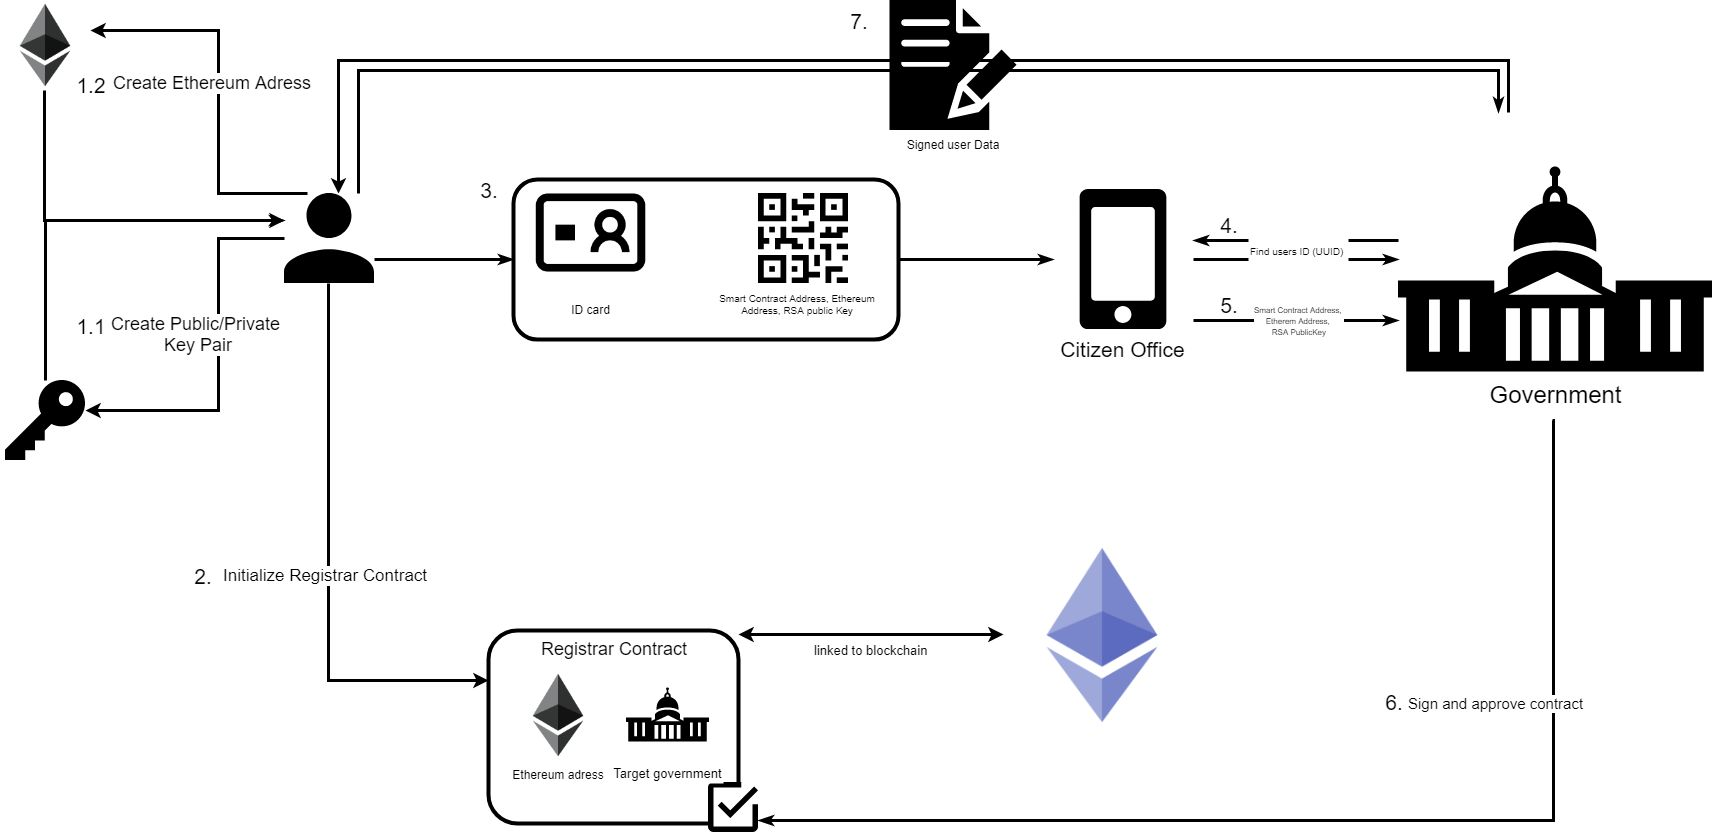
\includegraphics[width=\textwidth]{concept/registration_contract_general}
\caption{Registration}
\label{fig:registration_concept}
\end{figure}

\begin{enumerate}
\item \label{registrar_item_one}
The user creates an Ethereum address and a private public key pair, the combination of these two are now used as the users digital identity. Jointly they act as a digital identity card. They are safely and securely stored in the users own database.
\item \label{registrar_item_two}
For verification and auditing purposes these have to be verified by a trusted party, so that third parties can be sure of the identity of the individuals.
We are using a specially designed smart contract, where the user inputs his Ethereum address and his public key. Once filled, he writes it to the blockchain and waits for the trusted party, in our case a governmental agency, to check the contents, fulfill and sign the contract.
\item \label{registrar_item_three}
In order for that to happen, the user has to physically visit his citizen office with pre-existing identification documents. After verifying himself to the authorities they can use a specifically generated QR code to quickly check his digital identity.
\item \label{registrar_item_four}
With the information that is contained within the QR code the citizen office can now check their database for the corresponding entity.
\item \label{registrar_item_five}
After finding a corresponding user they extend their existing entity with the newly gathered Ethereum address, the users RSA public key, and the registration contracts Ethereum address.
\item \label{registrar_item_six}
The second to last step now is signing and approving the citizens registration contract.
\item \label{registrar_item_seven}
After approving the users registration contract the government creates a data blob containing all of the users information, signs it and lastly sends this signed user data to the user.
\end{enumerate}
The user is now a fully registered member within our community. Henceforth he can use this identity to request services and offer claims to and from other registered parties. 

\subsection{Permission Request}
\label{ssec:PermReq}
With registration complete it is now time to use the system for its intended purpose. Meaning requesting services or purchasing goods from providers such as Banks, 
Car Rental Agencies, Airlines using \projectName{} for verification. In order to better understand how \projectName{} facilitates these transactions it is important to understand that
each identity is defined by an enormous amount of characteristics. These could be, but are not limited to, their given name, family name, age, full address, employer, e-mail address, physical characteristics such as facial structure, eye color, etc.
Each of these is mapped to a single so called claim within \projectName{}. In detail a claim represents a manifestation of one of these attributes. For example their given name could be Andrew or their eye color could be blue.
However just mapping these attributes to claims is not enough, they have to be verified by a trusted entity. To not set unrealistic expectations we focussed on information that has already been verified by the government in the form of an id card or other easily verifiable information such as
e-mail addresses. Lets continue on to the actual flow of how these claims are exchanged and afterwards there will be a brief explanation for why this flow was designed as shown. 

\begin{figure}[ht]
\centering
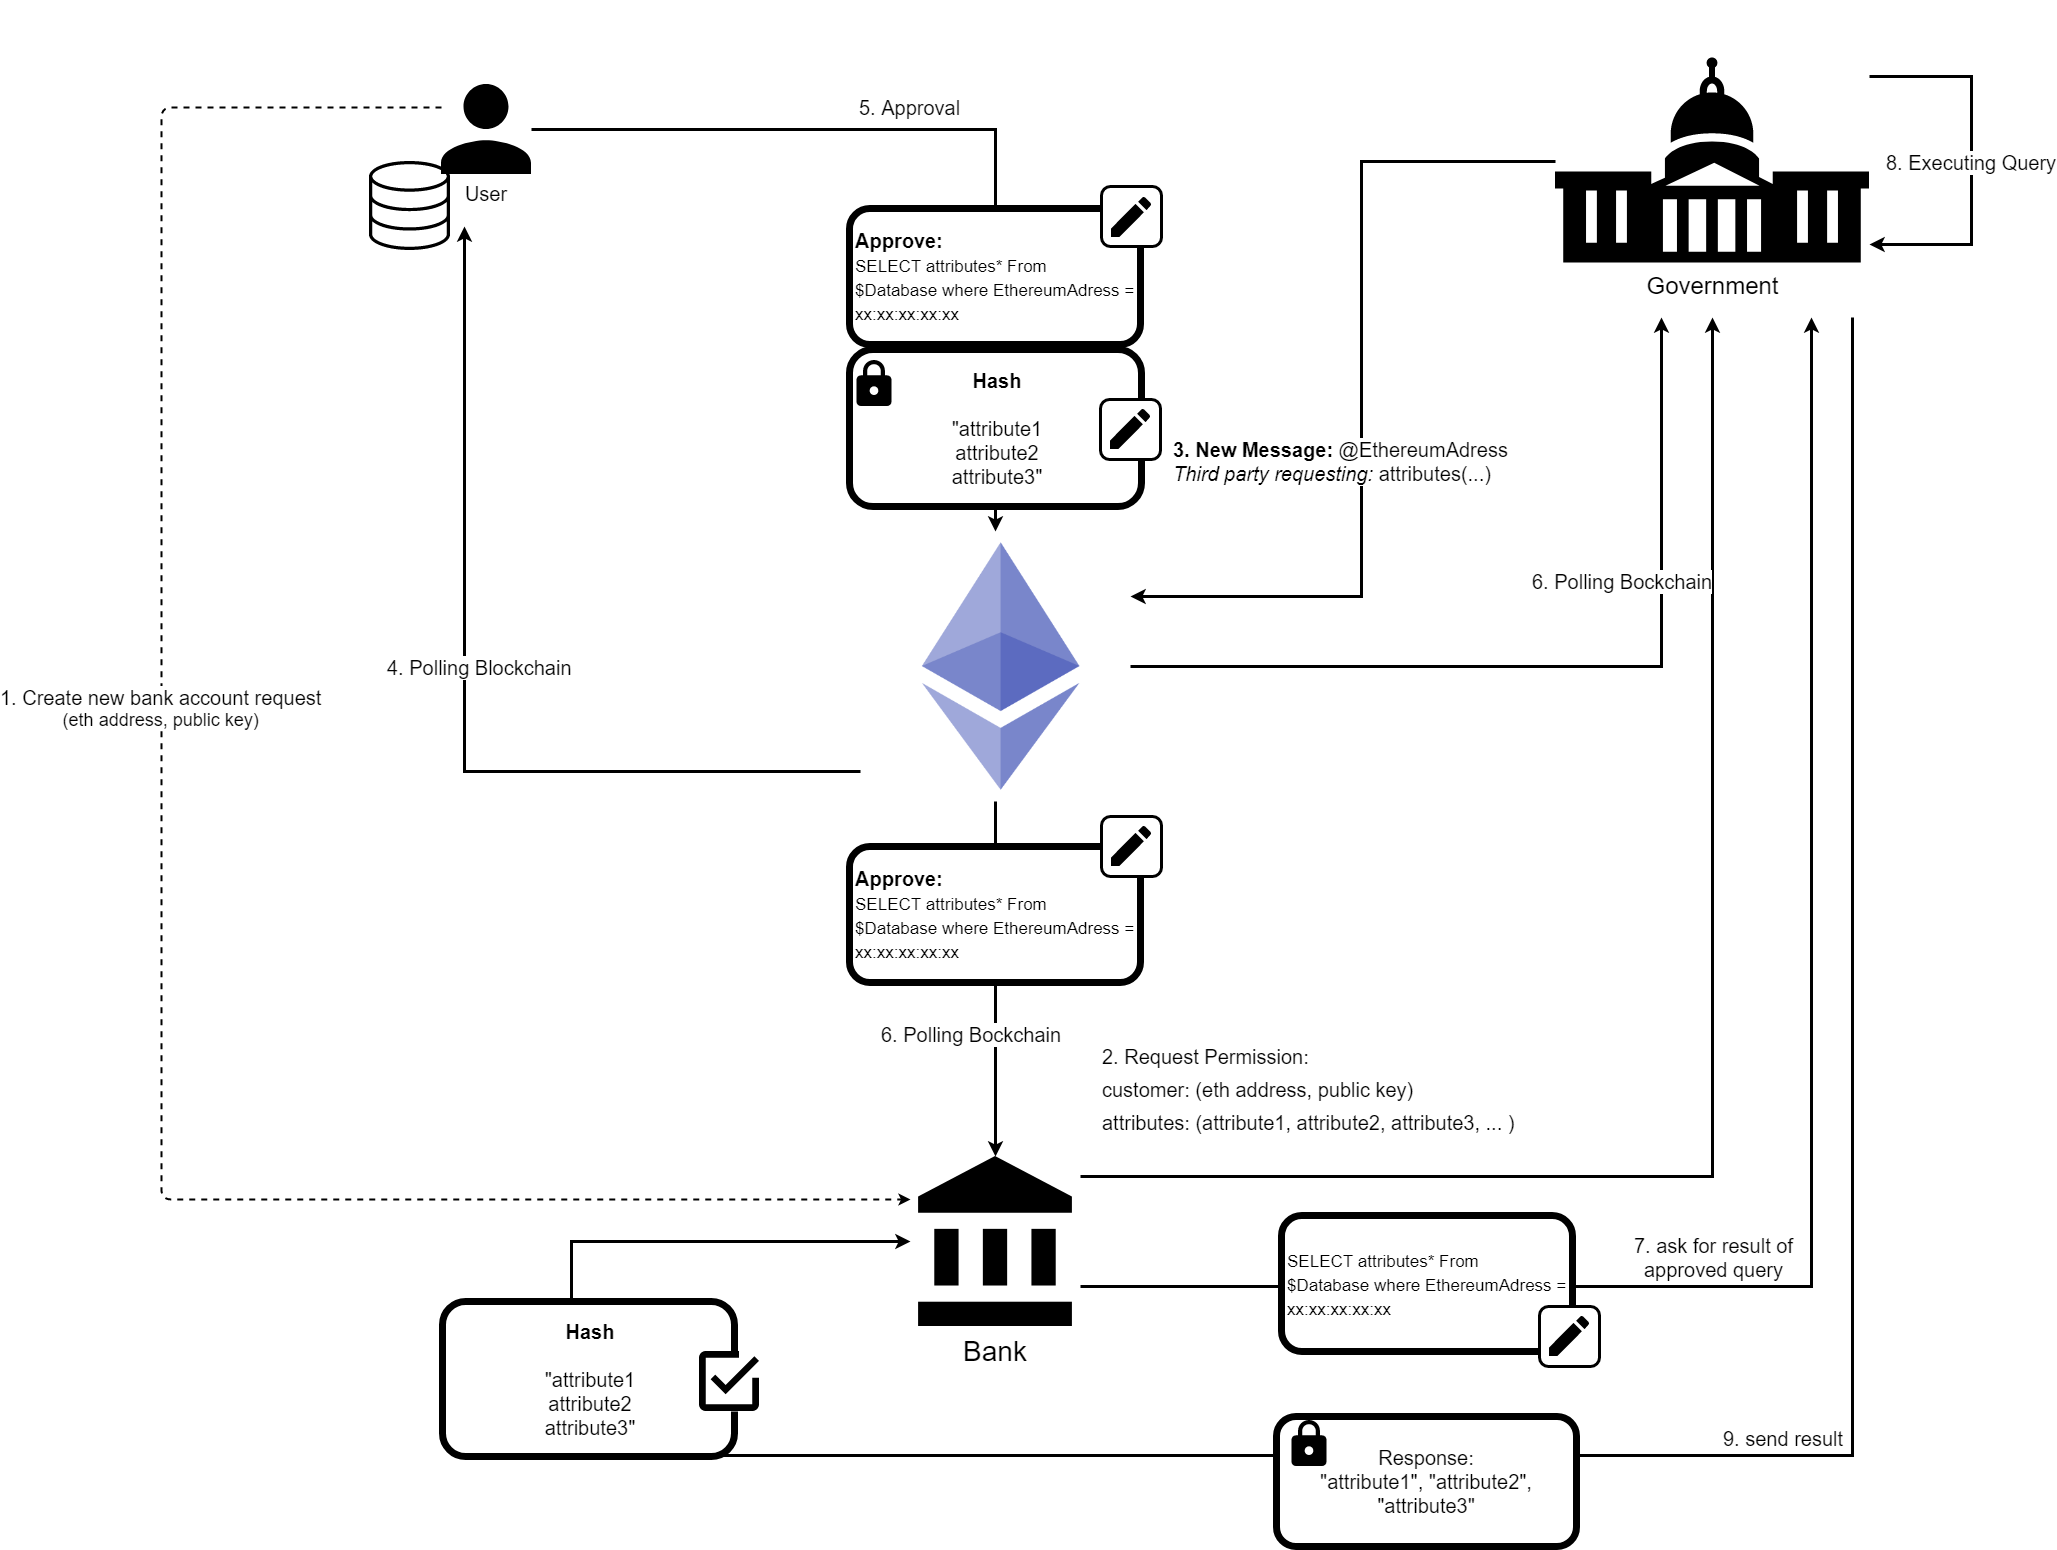
\includegraphics[width=\textwidth]{concept/permission_contract_general.png}
\caption{Permission Request}
\label{fig:permission_request}
\end{figure}

\begin{enumerate}
\item \label{permission_request_item_one}
The first step consists of a user requesting an actual service with his Ethereum address and public key, in this example we are examining the creation of a new bank account.
\begin{comment}
"An" goes before all words that begin with vowels:
An egg
With two exceptions:
When "u" makes the same sound as the "y" in you, or "o" makes the same sound as "w" in won, then "a" is used:
a union
a united front
a unicorn
a used napkin
a U.S. ship
a one-legged man
https://english.stackexchange.com/questions/105116/is-it-a-user-or-an-user
\end{comment}
\item \label{permission_request_item_two}
The bank teller now enters that information into a \textbf{Request Permission} form additionally containing all claims that they deem necessary. These may contain claims such as
family name, given name, date of birth, current address, etc. After completion of the form it is sent to our trusted entity, the government, for further processing.
\item \label{permission_request_item_three}
The government now checks whether this user is part of \projectName{} and if successful creates a new message containing the target users Ethereum address, requested claims and entity requesting the claims.
Therefore the message is loosely structured as follows:
\begin{itemize}
\item \textbf{EthereumAddress:} This is the users Ethereum address
\item \textbf{ThirdPartyName:} The Banks name
\item \textbf{Requested claims:} Actually contains two separate arrays.
One holds all the required claims, without which the bank account registration will fail and the other contains optional claims.
These optional claims might be additional information that the bank would like to have for their data storage, but which also is not integral to creating a bank account.
\end{itemize}
\item \label{permission_request_item_four}
The user now polls the blockchain for new messages and finds this permission request by the bank.
\item \label{permission_request_item_five}
The user now checks each requested claim and decides whether he is willing to share these with the bank.
Since the claims importance, meaning whether they are required or optional, is visible, the user has full knowledge over his shared claims and information.
He may also decide that he isn't willing to share some required claims, knowing that his service request may be denied because of it.
\item \label{permission_request_item_five}
After this decision a signed query containing the shared claims and a signed hash of the shared claims is written to the blockchain.
\item \label{permission_request_item_six}
The government and bank notice the users answer and poll the blockchain for the new message.
\item \label{permission_request_seven}
The bank can now use the signed query to send it to the government for information retrieval.
\item \label{permission_request_eight}
The government checks the query against the blockchain and executes it.
\item \label{permission_request_nine}
After the query results are calculated the government sends a signed object containing the claims and their values, and a signed hash of these to the bank.
\end{enumerate}
After fully exploring how a permission request works in \projectName{} it is important to explain some of the pecularities of the design.
\begin{itemize}
\item \label{design_pecularity_one} \textbf{Why is it so convoluted?}
This is in part because it was our utmost priority to keep the users data as secure as possible while still allowing for information to be shared digitally.
This is however not just motivated by our own beliefs and opinions, but also because of the upcoming GDPR\ref{subsubsec:GDPR_compliance} regulation.
\item \label{design_pecularity_two} \textbf{Why use the blockchain at all if only a small amount of the user base is allowed to write to it?}
The main advantage of blockchain technologies are that they are based upon an open ledger concept. This basically means that every entity that is part of the network has full access to all entries in the blockchain.
This enables every entity to check for the flow of information and whether a transaction actually took place. Lastly all information that has been written is immutable which enables every participant to verify whether they are dealing with
fraudulent or correct information.
These concepts enable our system and allow us to stay within the tight regulations of the GDPR\ref{subsubsec:GDPR_compliance} while still offering identity services. Using the blockchain for transactional information instead of identity information
secures a users right to privacy while allowing him to share his information with third parties. Since third parties have read access, they can verify whether their requests have actually been sent to the user they are in contact with and
whether that user agreed to share his information with the third party.
In conclusion using the blockchains immutability and open ledger principles third parties can be sure that their requests have been handled and responded to, without the possibility of tampering after writing.
This enables every participant to acknowledge that some form of claim sharing has occured and is therefore verifiable.
Furthermore writing a permission request to the blockchain removes the possibility for third parties to alter their information requests after they have been sent and therefore increases the users trust in the system.
Mainly because users now have to give explicit consent to each and every single claim that is being requested without the possibility of third parties intervening and adding claims to the request after they have been granted or denied.
\item \label{design_pecularity_three} \textbf{Are there any additional benefits to handling information this way?}
The signed queries could be enriched with flags to increase functionality and usability. For example a user might define a query to only be usable x times or only to be valid up until a specific date in the future.
This further reinforces his right to self-sovereignity by only allowing access to his information for a limited time. 
\item \label{design_pecularity_four} \textbf{What are the costs associated with this process for the user?}
Users don't pay for the creation of the smart contract handling this information sharing request. However should claims change that have been shared as part of a permission request contract the user is financially responsible for the transaction costs of changing these signed claims.
\end{itemize}

% Please agument why the user if he is holding signed claims is not providing his claims directly to the requesting provider
% Include the following arguments:
% 1. request shall be populated through the blockchain so that every entity can acknowledge the claim sharing
% 2. populatring thre reuqest through the blockchain gives us the possibility to explicit approve the sharing
% 3. generating a signed query can also have additional attributes like a reuse flag to indicate if the query could be used again if the claim changed
% 4. user don't have to pay for the creation of the smart contract. only for the updating of the signed values



\subsection{Closures}
\begin{figure}[ht]
\centering
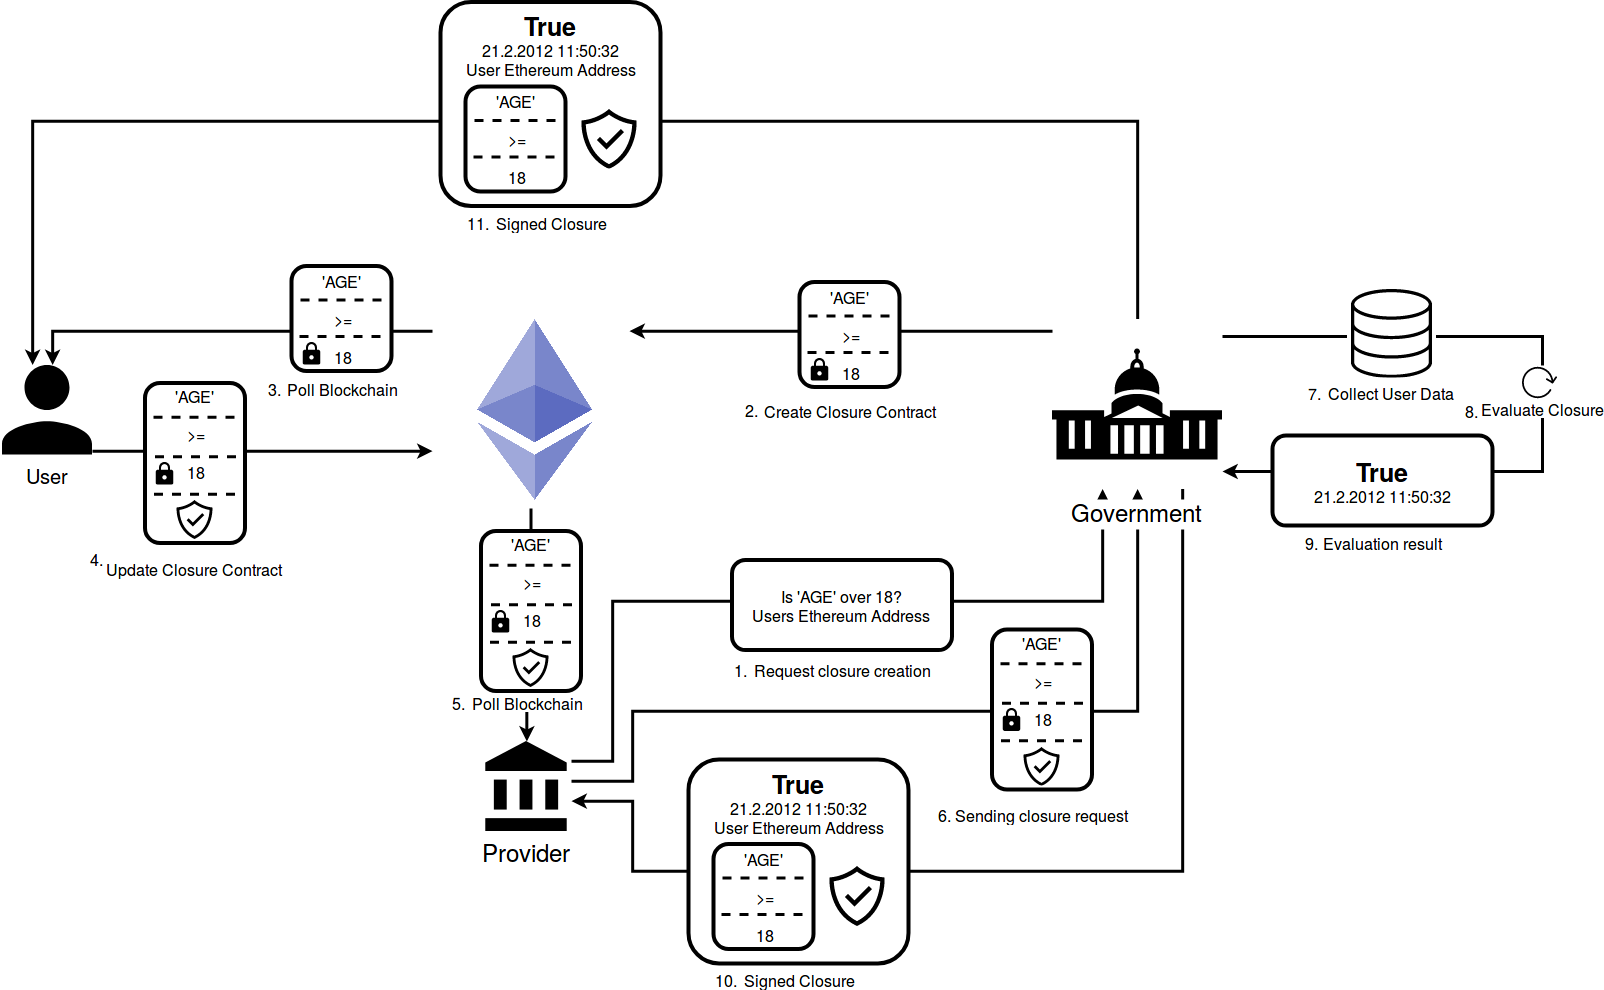
\includegraphics[width=\textwidth]{concept/closure_contract.png}
\caption{Closure Contract}
\label{fig:closure}
\end{figure}

To introduce the concept behind \textit{closures}, lets say a web content provider wants to know if the user is over 18 years old to be allowed to visit a web page. Since the provider does not need to know the exact age of the user to evaluate this expression, he can trust someone that is already holding that information of the user, who then can evaluate if the user is over 18 years old and provide the result of that query, in a verified manner, to the requesting provider. This procedure enables us to “hide” the real value of the identity attribute of the user, while still providing certified information. In our case the government evaluates this closure expression since it is a trusted entity. In general every provider holding that identity value could evaluate the closure. However the trustworthyness of that result is at most of the same level as the trustworthyness of the provider or lower.

\noindent Closures are designed to contain five core elements:
\begin{enumerate}
\item \textbf{Closure expression:} The expression over a user’s identity attribute identifier, a logical comparison operator and the comparison value. For example: “’AGE’, greater then, 18 ?”
\item \textbf{User Ethereum Address:} References the user that is the subject to this closure
\item \textbf{Evaluation result:} Either “true” or “false”, depending on the evaluation result of the closure expression. Evaluations, once created, are not updated even if the user’s attribute changes.
%https://english.stackexchange.com/questions/104740/created-at-or-created-in
\item \textbf{Creation date:} The date this closure was created on. Providers can decide if they need a new closure because the creation date is too far in the past.
\item \textbf{Signature:} The signature over all of the above entries. This signature is issued by the entity that evaluated the closure.
\end{enumerate}

Let us start by glancing at the closure requesting and creation flow as displayed in figure \ref{fig:closure}. We start off at the provider requesting a closure over the age of the user in step 1.
The provider is referencing the user by his ethereum address so that the government that creates the closure contract, knows whom to address this contract to. In step 2 the government creates the “Closure Contract” containing the users attribute identifier “AGE”, the logical comparator “>=” (greater or equals) and the asymmetrically encrypted comparison value “18”.

Since the blockchain is public, every observing party could notice this new closure contract. If the comparison value was not encrypted, we would expose semi-critical personal information about the user, even without populating the closure evaluation result through the blockchain. Imagine a longterm passive adversary that is observing closure contracts. This adversary could learn valuable Information about specific users from mapping closure requests to users over a long time period. Imagine a user that is using fixed rate payments often while shopping. So the provider would create a corresponding amount of closure requests concerning the users bank account to validate his liquidity. One closure over “>1.000\$ ?”  another one over “> 5.000\$” and lastly over “> 12.000 \$”. The adversary could learn that even without knowing the closure evaluation result that the users bank account is likely at least over 5.000\$ since the provider requested the 12.000\$ closure last. This would help an adversary to find valuable targets.
To conclude we prevent this type of long-term observation attacks by encrypting the comparison value, so that only the user can encrypt this value.

However, in step 3 the user is pulling the new closure contract, decrypting the closure comparison value, and if he approves the closure generation, signs the closure requests and updates it in the blockchain (step 4). He would further proceed by encrypting the closure comparison value again, now with the public key of the provider which initially requested the closure. The provider is receiving the updated, signed closure request in step 5.

Note that the closure is still not evaluated, and now only an approved closure request. Even if the user could evaluate the closure he does not have the necessary level of trust to provide a trustworthy closure. Self generating a closure concerning himself would be equivalent to signing a paper claiming to be over 18 years old.

After the provider validates the signature of the closure request, he uses this approved closure creation request to query the government for the closure expression result (step 6). The government is again validating the signature of the closure, verifies that the user indeed granted his approval and queries its database for the users identity information (step 7). Now the closure can be evaluated on the actual identity information (step 8) and a closure evaluation result is generated (step 9). Additionally we save the current time stamp in conjunction with this evaluation result, since identity information may change, but the closure evaluation result remains the same. Since closures are stateless they could be reused by every closure holder. Depending on the creation date each provider can decide whether to accept the closure or request a new one with updated identity information.\footnote{While this makes no sense when getting a closure over the “age greater equals 18” that evaluated to “true”, it makes sense to request new closures on attributes that are fluctuating more often like bank accounts.}

The government now creates a real closure by mapping the closure request, closure evaluation result and creation date together. It further creates a signature over these values to ensure the closures integrity, but more importantly to establish trust. Each entity receiving this closure can validate the signature and decide weather to trust it depending on the trust level of the issuing provider. In step 10. the requesting provider receives a copy of the closure so that he can use the closure evaluation result to either deny access to the web content or allow the user to proceed. Finally the user also receives a copy of the closure which he may use to provide to other entities as well, so we don’t need to generate a new closure each time the same closure is requested.

To conclude the closure creation flow lets us answer why the closure request needs to be populated through the blockchain. First we ensure non-repudiation, since the provider can't deny having received the closure creation approval and the user can't deny having approved this closure creation. Second and more important is that each entity with access to the blockchain can see what information a provider is requesting. This would make the anonymized data collection process much more transparent. And third we ensure that the government asks the user for his explicit approval before creating the closure.

\subsection{Changing Claims}

\begin{figure}
 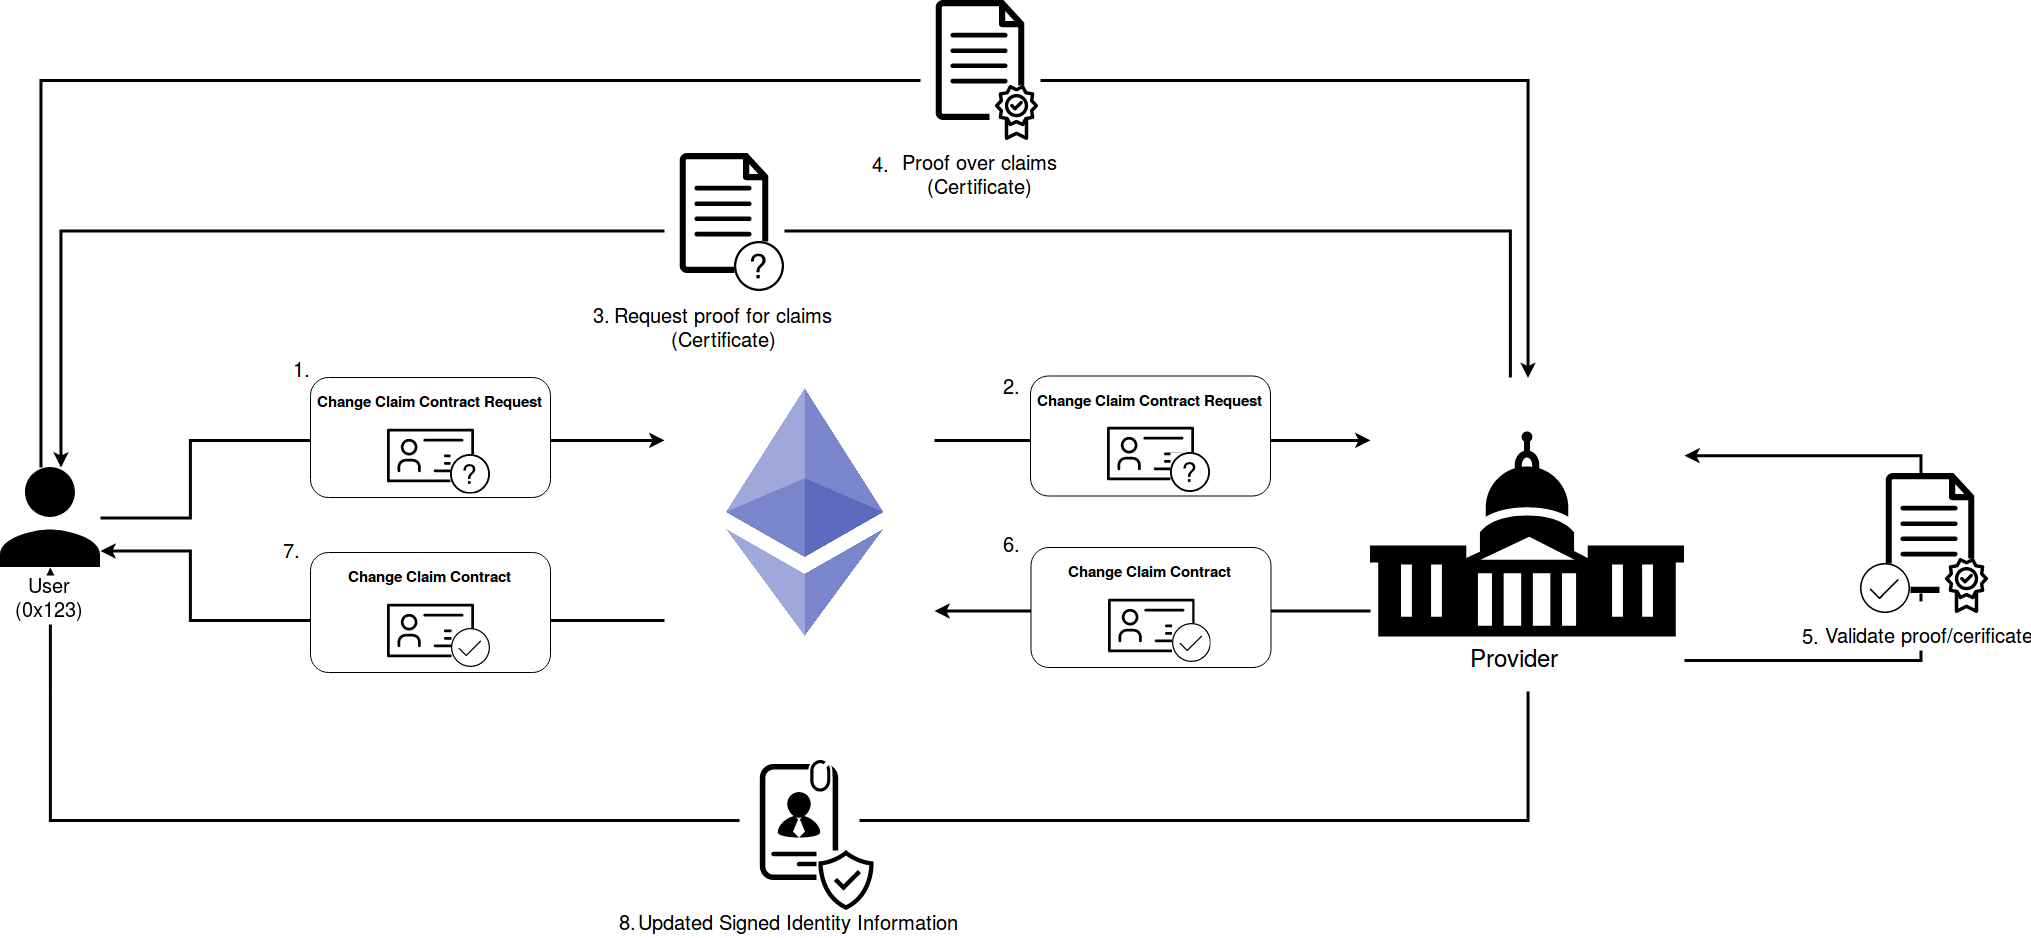
\includegraphics[width=\textwidth]{concept/change_claim.png}
 \centering
\caption{Concept of the change claim work flow. Change claim events are populated trough the blockchain so that every provider holding the same claim for the referenced user can start a new permission request to update the claim values.}
\label{fig:changeClaimsFig}
\end{figure}

Changing claims in a self-sovereign manner while still providing the high levels of trust in these claims is a challenge. We evaluated two entry points for this contract: a) the user starts the procedure by sending a “change claim contract request” or b) the government enforces new claims by populating a “change claim contract”.

Both actions are described as use cases in section \ref{sec:changeClaimUseCase}. For a) the use case that the user may want to change his family name because he got married recently. In the case of b) the government triggers a change claim as a law enforcement action (e.g. the user looses his driving license for a certain time) or anoother federal institution wants to update the users claims. Each scenario is described in detail in this section.

To still serve as a self-sovereign system the user has the ability to create a “change claim contract request” (step 1, figure \ref{fig:changeClaimsFig}). This contract itself does not enforce any change of any attributes, but serves as a change claim application. The user states the claim IDs he wants to change within the contract. He may even add additional attributes like a time period to define for how long the claim shall be changed. It is also possible to propose new claims the user wants to add by himself. However, new or changed claims need to be verifiable by the provider. The “change claim contract request” is likely addressed at the institution that would have the highest trust level of all entities within the system, since the signature over these claims is only trusted as highly as the institution itself. In our scenario the government satisfies this trust level. Some might argue that it is not necessary to populate the “change claim contract request” through the blockchain (since each transaction costs money), but it helps to establish more transparency in our system and relocates power to the user. He decides which claims he wants to change and which new claims he wants to have added to his digital identity.

The government pulls the “change claim contract request” from the blockchain and evaluates it in step 2, which claims it needs a verification for, e.g. a certificate. Off-blockchain the user is asked for proof or certificate over his proposed claims (step 3). Each provider can define which kind of proof the user must provide to get his claim changed. The level of trust in a provider grows with the amount of accuracy the provider puts in his claim validation. The user provides the proof in step 4. Since different providers may accept different proofs, it can be comprised of various documents, like photos of his ID card, certificates of his club membership or even audio recordings. However, if the user is not able to provide the necessary proofs, the contract will be terminated and the change claim request rejected.
The provider validates if the provided proofs satisfy his acceptance criteria in step 5.  If the proofs are sufficient the provider accepts the “Change claim contract request” by setting a flag in the contract, or even removing some claims from the contract for which the verification failed (step 6.).

Now every other provider in the system holding old claim values for the referenced user can create a new permission request to discover the newly changed claims from the provider handling the change claim contract. The user still needs to approve the new incoming permission requests. In step 7 the user gets the notification about the successful approval of the change claim contract and queries the provider to retrieve a signed version of his updated claims (step 8.).

Now the change claim process is finished. However, as mentioned previously there is also a scenario where a federal institution wants to enforce a claim change (for example the temporary removal of a driving license). In that case we would directly start at step 6 where the government will publish an already approved “change claim contract” referring to the claim IDs that were changed and additional values restricting the duration of this enforcement. External observers of the blockchain will notice that it is a forced claim change since the user did not provide a “change claim contract request”. In the same way as described previously, the provider will take note about the claim change and can setup a new permission request to discover the new claims. As a side note: If the user rejects the permission requests the providers holding outdated claim values can simply distrust these values and decide if they are still willing to render services to that specific user. Please refer to section \ref{sec:changeClaimUseCase} for a use case.

\subsection{Evaluation}

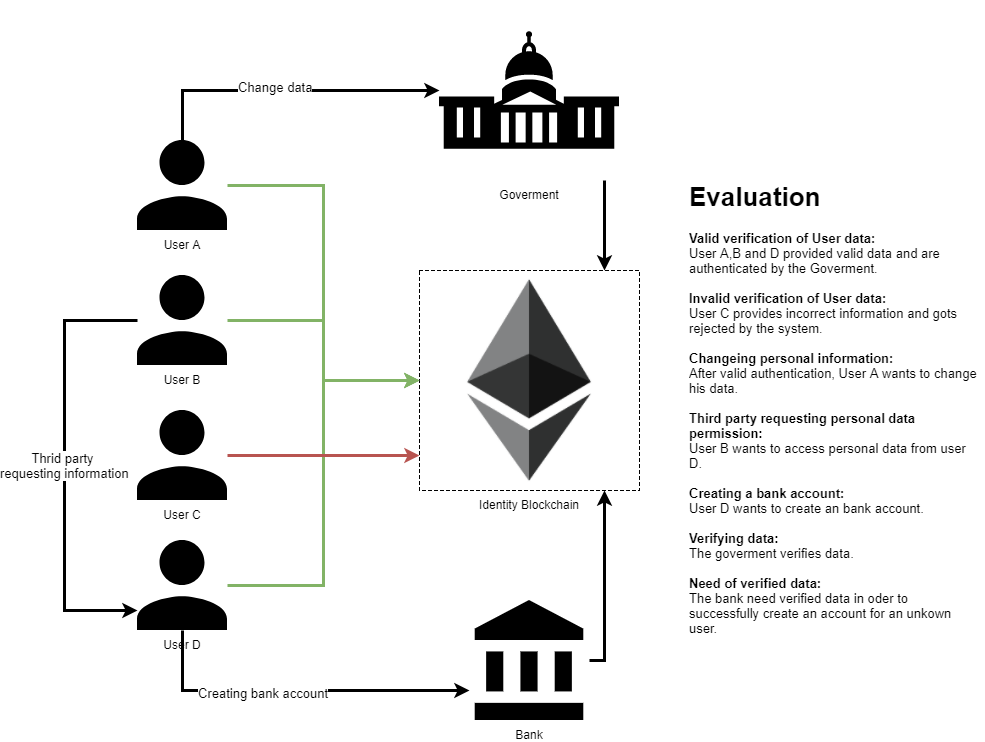
\includegraphics[width=\textwidth]{concept/evaluation.png}
 
\section{Use cases}

\subsection{Registering with the system}
\label{ssec:registerWithSystem}
To demonstrate how our system works we will try to formulate a specific use case, in order to provide an example. An additional prerequisite we will define is that \projectName{} has been deployed by a centrally trusted entity like the government.

Lets consider aunt Trudy who is not very technologically knowledgeable. In order to refresh her identity card she visits the citizen center closest to her and the teller at the register informs her about a new digital identity service that can offer digital verification for a multitude of plattforms that Trudy frequents. She decides to give it a try since the teller informs her that it is conforming to the GDPR\cite{gdpr}.

Because registration is quick and easy she decides to do it right there on the spot. She downloads the app and enters a name of her choice and decides on a password. The system now generates a new user account with Trudy's chosen settings. This sets up the "register contract" within the ethereum network containing her information.\ref{ssec:PermReq} After she is logged in, which happens automatically after the registration process, the teller asks Trudy to open her personal Dashboard and click on "Show QR-Code". The teller then scans this QR-Code with a special app which then parses the information within the QR-Code and finds the corresponding registration contract within the blockchain. Now this the information within this contract is compared to the information within the QR-Code and either verified and approved, or denied.

Now Trudy is part of the system and is ready to participate within the \projectName{} ecosystem. Additionally she got sent all available claims and can easily check which information she can share with other members.

\subsection{Requesting permission from a user}
\label{ssec:requestingPermission}
In order to try out the system Trudy now decides to create a new bank account with a newly established heavily marketed bank. After waiting in line, it is finally her turn to speak with the bank teller. She tells her, that she would like to create a new bank account using \projectName{}, which is no problem at all. The teller asks her for her ethereum address and her public key, which is easily shared through nfc or comparable protocols.
The teller enters her ethereum address into the registration form and waits for the available claims to arrive . Now the teller can decide on claims that are required and optional and sends the form to the government.
The government now checks for that ethereum address within its record and whether it is associated with an active user. After finding Trudy, it writes a new message in the form of a smart contract to the blockchain containing Trudy's ethereum address and the request containing all required and optional attributes.
Trudy's app automatically polls the blockchain every of couple seconds and notifies Trudy about a new permission request containing all Attributes the Teller requested. She now decides which information she is willing to share and which she isn't. After she is done deciding, the information is written in a new message to the blockchain, containing the information she approved for sharing purposes.
The government also automatically polls the blockchain every couple of seconds and notices an answer to the previously created permission request.
The Bank also has read access to the blockchain and notices the answer aswell. The Bank now takes the message containing the approved attributes and sends them as query to the government.
The government verifies whether the query sent by the bank matches the one Trudy approved and if they are equal, the government queries its database and creates a result, which is then sent to the Bank.

Now the teller informs Trudy of a successful sharing of claims and starts introducing Trudy to the Banks general rules and regulations, as she is now a new customer.

\subsection{Change a claim}
\label{sec:changeClaimUseCase}
\textbf{a) User changes claims:}
Lets have a user Bob Bobsen who has recently married Alice Alicon. Since Bob wants to change his family name to Bob Alicon this information needs to be updated in our system. To do so he creates a new “Change Claim Contract Request” holding the “FAMILY\_NAME” claim ID and addressing this contract to the government. The government will ask Bob for his marriage certificate. Bob sends his certificate over a secured connection to the government. They, on the other hand, can now verify the new claim by checking Bob's marriage contract. If the certificate is authentic the identity provider publishes an approve transaction to the change claim contract to notify all third parties and other identity providers about the new claim of Bob's digital identity.
Bob then pulls the blockchain, and requests the signed version of his new family name from the government, which he saves in his local database.

\textbf{b) Enforced claim changes:}
Bob has lost his driving license by committing a traffic violation. Since Bob is still holding a signed version of his driving license in his local database he could easily rent a new car. So the government enforces a claim change by publishing a “Change Claim Contract” to the blockchain referencing Bobs ethereum ID, the driving license claim ID and a time period (6 months) during which his license is suspended. Each entity observing the blockchain now knows that the driving license claim value provided by Bob has been suspended for 6 months, if the provided signature is older then the creation date of the “Change Claim Contract”. However, Bob can query the government for the updated claim value and retrieve the temporary restricted driving license, which is then also trusted, because it is up to date. After 6 months no new claim change contract needs to be setup because an entity can simply compute that the suspension time is expired and that no new claim change was published by the government.
